\chapter{Momentum Transport}

\section{基本数学知识}
\subsection{大学白学了}

\[\frac{d}{dx}(uv) = u\frac{dv}{dx} + v\frac{du}{dx}\]

\subsection{矢量计算}

几个基本的等式:

\[\nabla s = \frac{\partial s}{\partial x}\bm{i} +  \frac{\partial s}{\partial y}\bm{j} + \frac{\partial s}{\partial z}\bm{k}\]

\[\nabla\cdot\bm{u} = \frac{\partial u}{\partial x} + \frac{\partial v}{\partial y} + \frac{\partial w}{\partial z}\]

\[\nabla^2\bm{u} = \frac{\partial^2 u}{\partial x^2} + \frac{\partial^2 v}{\partial y^2} + \frac{\partial^2 w}{\partial z^2} \]

\[\nabla\cdot (s\bm{u}) = s\nabla\cdot\bm{u}+\bm{u}\cdot\nabla s\]

\subsection{Gauss散度定理}
整个控制体内的源汇项=控制体表面的净通量:

\begin{equation}\label{Gauss}
\int_{V}(\nabla\cdot \bm{u})dV = \int_{S} (\bm{u\cdot n})dS
\end{equation}

\subsection{Leibniz积分法则}

给出了一个对积分变量为函数的积分求导的法则,右侧第一项解释了积分随时间的变化,二三两项区域内物理量的得失。

\begin{equation}
    \frac{d}{dt} \int_{a(t)}^{b(t)} \phi(x,t) dx = \int_{a(t)}^{b(t)} \frac{\partial \phi}{\partial t} dx + \phi(b(t),t) \frac{\partial b}{\partial t} - \phi(a(t),t)\frac{\partial a}{\partial t}
\end{equation}

对由面$ S(t) $包围的封闭三维空间$ V(t) $来讲,假设面的移动速度为$ \mathbf{v_s} $,有如下积分法则:

\begin{equation}
    \frac{d}{dt} \int_{V(t)} \phi dV = \int_{V(t)} \frac{\partial \phi}{\partial t} dV + \int_{S(t)} \phi(\mathbf{v_s}\cdot \mathbf{n}) dS
\end{equation}

若控制体不移动,则:

\begin{equation}\label{Leibniz}
\frac{d}{dt} \int_{V(t)} \phi dV = \int_{V(t)} \frac{\partial \phi}{\partial t} dV
\end{equation}

\subsection{Reynolds输送定理}
Reynolds输送定理可用来定量地描述流场中流体性质的变化情形,譬如在一个控制容积(Control volume)之中含有某种流体。在经过一段时间之后,若控制容积中流体的总体性质B有所改变,则其变化必定是下列两种原因所造成的:

(1)总体性质B可能会因为本身的特性或外在因素的影响而产生随时间的变化,譬如流体中含有某种化学物质,该物质会因化学反应造成其质量B的变化,$ dB/dt $即为该物质质量的变化率。又譬如B为流体的动量,在受到外力的状况下,流体的动量会有所改变;

(2)因为流体流动所造成的变化:当流体流经控制容积时,会带入或带出一部份的物质。当流出控制容积的总体性质大于流入量,则净流出量为正,会造成控制容积之中该总体性质的减少;反之,流入量大于流出量便会造成该总体性质的增加。


对固定控制体来讲:

\begin{equation}
    \left( \frac{dB}{dt} \right)_{MV} = \int_V \frac{\partial}{\partial t}(b\rho)dV + \int_S b\rho\mathbf{v\cdot n} dS
\end{equation}

运用Gauss散度定理(\autoref{Gauss})简化形式:

\begin{equation}
    \left( \frac{dB}{dt} \right)_{MV} = \int_V \left[ \frac{\partial}{\partial t}(\rho b) + \nabla\cdot(\rho b\mathbf{v}) \right]
\end{equation}

配合随体导数和矢量计算可写成:

\begin{equation}
\left( \frac{dB}{dt} \right)_{MV} = \int_V \left[ \frac{D}{Dt}(\rho b) + \rho b \nabla\cdot\mathbf{v} \right]
\end{equation}

\section{无量纲数}\label{dimensionless-number}

Reynolds Number,定义为惯性力和粘性力的比:

\[ Re = \frac{\rho UL}{\mu} \]

Grashof Number,定义为浮力和粘性力的比,$ \upsilon $为动力粘度:

\[ Gr = \frac{g\beta\Delta TL^3}{\upsilon^2} \]

Prandtl Number,定义为动量扩散率和热扩散率之比(也代表流动边界层和热边界层之比),$ k $为导热系数,$ \alpha $为热扩散系数,$ \upsilon $为动力粘度。随着$ Pr $增大,热对流的增大速率逐渐比热传导大:

\[ Pr = \frac{\mu c_p}{k} = \frac{\mu/\rho}{k/\rho c_p} = \frac{\upsilon}{\alpha} \]

P\'{e}clet Number,定义为对流传递速率与扩散传递速率之比,$ D $为质量扩散系数:

\[ Pe =
\begin{cases}
\frac{\rho ULc_p}{k} = \frac{UL}{\alpha} = RePr & \text{for heat transfer}\\
\frac{UL}{D} = ReSc & \text{for mass transfer}
\end{cases}
\]

Schmidt Number,定义为动量扩散率和质量扩散率之比:

\[ Sc = \frac{\upsilon}{D} \]

Nusselt Number,定义为对流和热传导之比:

\[Nu = \frac{hL}{k}\]

Mach Number,定义为速度和介质中声速之比:

\[ M = \frac{|\mathbf{v}|}{a} \]

声速由下式计算,其中$ \gamma=c_p/c_v $为比气体常数:

\[a=\sqrt{\gamma\left( \frac{\partial p}{\partial \rho} \right)_T}\]

对理想气体而言,简化如下:

\[a=\sqrt{\gamma RT}\]

Eckert Number,动能和焓之比。如果$ Ec\ll 1 $,能量方程中的粘性耗散和压力功就可以忽略(事实上这个无量纲数就是为了表明,在速度不太高的情况下,可压缩流体的的粘性耗散和压力功可以忽略):

\[Ec=\frac{\mathbf{v\cdot v}}{c_p\Delta T}\]

Froude number,定义为特征速度和重力波速度之比,用来表征固体在流体中运动的情况,$ Fr $越高意味着固体所受阻力越大:

\[Fr = \frac{U}{\sqrt{gL}}\]

Weber Number,定义为惯性力和表面张力之比:

\[We=\frac{\rho U^2 L}{\sigma}\]

\section{常见物理量}

粘度$ \mu $,单位\si{\pascal\per\second},定义为剪应力与剪切速率之比。

\[\tau = \mu\frac{\partial u}{\partial y}\]

动力粘度,单位\si{\meter\squared\per\second},定义为粘度与密度的比值。

\[\upsilon=\frac{\mu}{\rho} \] 

\section{随体导数}
微元中的物理量$ \phi $是位置和时间的函数,单位质量的物理量的变化率$ D\phi/Dt $定义为:

\begin{equation}
\frac{D\phi}{Dt} = \frac{\partial \phi}{\partial t}+\frac{\partial \phi}{\partial x}\frac{dx}{dt} + \frac{\partial \phi}{\partial y}\frac{dy}{dt} + \frac{\partial \phi}{\partial z}\frac{dz}{dt}=\frac{\partial \phi}{\partial t}+u\frac{\partial \phi}{\partial x}+v\frac{\partial \phi}{\partial y}+w\frac{\partial \phi}{\partial z}=\left[\frac{\partial \phi}{\partial t}+\bm{u}\cdot \nabla \phi\right]
\end{equation}

守恒方程的通用形式为:

\begin{equation}
\frac{\partial \rho\phi}{\partial t}+\nabla\cdot(\rho\phi\bm{u}) = 0
\end{equation}

\section{连续性方程}
由随体导数很容易推导关于物理量密度$ \rho $的守恒方程:

\begin{gather}
\frac{\partial \rho}{\partial t} + \frac{\partial \rho u}{\partial x} + \frac{\partial \rho v}{\partial y} + \frac{\partial \rho w}{\partial z} = 0 \\
\frac{\partial \rho}{\partial t} + \nabla \cdot (\rho\bm{u}) = 0
\end{gather}

\section{动量传递}
\subsection{Non-Conservative Form}
由随体导数的Reynolds输送定理可推导出:

\begin{equation}
\int_{V}\left[ \frac{D}{Dt}(\rho\bm{u}) + (\rho\bm{u}\nabla\cdot \bm{u}) - \bm{f} \right]dV = 0
\end{equation}

即:

\begin{equation}
\frac{D}{Dt}(\rho\bm{u}) + (\rho\bm{u}\nabla\cdot \bm{u}) = \bm{f}
\end{equation}

用微积分基本定理拆开,发现2、3两相就是连续性方程(不信自己拆),等于0:

\begin{equation}
\rho\frac{D\bm{u}}{Dt}(\rho\bm{u}) + \underbrace{ \bm{u}\frac{D\rho}{Dt} + \rho\nabla\cdot\bm{u} } = \bm{f}
\end{equation}

然后得到非守恒形式的动量方程,其中$ \bm{f} $为各种力:

\begin{equation}
\rho\left[ \frac{\partial \bm{u}}{\partial t} + \bm{u}\cdot\nabla\bm{u} \right] = \bm{f}
\end{equation}

\subsection{Conservative Form}
用那个Gauss散度定理推出的Reynolds输送定理可推导出:

\begin{equation}
\int_{V}\left[ \frac{\partial(\rho\bm{u})}{\partial t} + \nabla\cdot(\rho\bm{uu}) - \bm{f} \right]dV = 0
\end{equation}

即:

\begin{equation}
\frac{\partial(\rho\bm{u})}{\partial t} + \nabla\cdot(\rho\bm{uu}) = \bm{f}
\end{equation}

写成常见的守恒形式,左边的为各种力$ \bm{f} $,其中$ \tau $为应力张量,$ F $为体积力:

\begin{equation}
\frac{\partial \rho\bm{u}}{\partial t} + \nabla\cdot(\rho\bm{uu}) = -\nabla\cdot p\bm{I} + \nabla\cdot\tau + F
\end{equation}

\section{应力张量}
动量方程中主要包括两种力,表面力(压力、粘性力)和体积力(重力等)。

\subsection{Surface Forces}
主要是压力和粘性剪应力。压力为正应力$ \tau_{ii} $,使有限控制体体积发生变化;粘性剪应力为切应力$ \tau_{ij} $,使有限控制体形状发生改变,但是体积不变;

故,应力张量可分为两个部分:

\[-p\bm{I}+\tau\]

\subsection{Body Forces}

重力:

\[\bm{f}_b = \rho \bm{g}\]

由旋转引起的Coriolis forces和Centrifugal forces

\section{牛顿流体的应力张量和动量方程}
对牛顿流体来讲,应力张量是剪应力的线性函数。

\begin{equation}
\tau = \mu\left(\nabla\bm{u}+(\nabla\bm{u})^T\right)+\lambda(\nabla\cdot \bm{u})\bm{I}
\end{equation}

对不可压流体来说$ \nabla\cdot\bm{u} = 0 $,动量方程的一般为:

\begin{equation}
\frac{\partial \rho\bm{u}}{\partial t} + \nabla\cdot(\rho\bm{uu}) = -\nabla p\bm{I} + \nabla\cdot(\mu\left(\nabla\bm{u}+(\nabla\bm{u})^T\right)) + F
\end{equation}

如果粘度为常数(一般等温会出现这种情况),动量守恒可进一步简化。无粘流体直接去掉粘度了事:

\begin{equation}
\frac{\partial \rho\bm{u}}{\partial t} + \nabla\cdot(\rho\bm{uu}) = -\nabla p\bm{I} + \mu\nabla^2\bm{u} + F
\end{equation}

\section{通用的守恒方程}
增加率+净流出=扩散增加率+源项

\begin{equation}
\underbrace{\frac{\partial (\rho\phi)}{\partial t}}_{\text{unsteady term}} +
\underbrace{\nabla\cdot(\rho\phi\bm{u})}_{\text{convection term}} =
\underbrace{\nabla(\Gamma\nabla\phi)}_{\text{diffusion term}} +
\underbrace{S}_{\text{source term}}
\end{equation}

在有限体积法中,会在整个控制体内对方程积分:

\begin{equation}
\int_{CV}\frac{\partial (\rho\phi)}{\partial t}dV + \int_{CV}\nabla\cdot(\rho\phi\bm{u})dV = \int_{CV}\nabla\cdot(\Gamma\nabla\phi)dV + \int_{CV}SdV
\end{equation}

然后用Gauss散度定理将对流-扩散项从体积分改为面积分,同时用\autoref{Leibniz}所示的Leibniz积分法则改写第一项。

\begin{equation}
\frac{\partial}{\partial t}\left(\int_{CV}\rho\phi dV\right) + \int_{A}\bm{n}\cdot(\rho\phi\bm{u})dV = \int_{A}\bm{n}\cdot(\Gamma\nabla\phi)dV + \int_{CV}SdV
\end{equation}

有限体积法的积分方程具有非常自然的物理意义,左边第一项表示物理量$ \phi $在控制体中的变化率,左边第二项表示控制体面上的净流出量(即对流项),右边第一项表示扩散引起的增量,最后一项为源-汇项。

对于稳态问题,时间导数为0:

\begin{equation}
\int_{A}\bm{n}\cdot(\rho\phi\bm{u})dV = \int_{A}\bm{n}\cdot(\Gamma\nabla\phi)dV + \int_{CV}SdV
\end{equation}

对瞬态问题,需要在每一个时间步内进行积分:

\begin{equation}
\int_{\Delta t}\frac{\partial}{\partial t}\left(\int_{CV}\rho\phi dV\right) + \int_{\Delta t}\int_{A}\bm{n}\cdot(\rho\phi\bm{u})dV = \int_{\Delta t}\int_{A}\bm{n}\cdot(\Gamma\nabla\phi)dV + \int_{\Delta t}\int_{CV}SdV
\end{equation}

\section{FVM 有限体积法}

基本思路:

\begin{enumerate}
    \item 将计算区域划分为一系列不重复的控制体积 ,每一个控制体积都有一个节点作代表 ,将待求的守恒型微分方程在任一控制体积及一定时间间隔内对空间与时间作积分 ;
    \item 对待求函数及其导数对时间及空间的变化型线或插值方式作出假设 ;
    \item 按选定的型线作出积分并整理成一组关于节点上未知量的离散的代数方程,使用代数方法求解。
\end{enumerate}

\subsection{对流-扩散问题的离散方式}

\begin{description}
    \item[一阶迎风] 一阶精度,绝对稳定,假设界面上的物理量和上游的物理量一样。可以获得物理上能接受的解,但当$ Pe $数较大时,假扩散比较严重,需要加密网格;
    \item[二阶迎风] 二阶精度,绝对稳定,边界上的物理量由上游的两个点插值得出。通用存在假扩散;
    \item[QUICK] 其对流项有三阶精度(用了三个数据点插值),扩散项仅有二阶精度(通常等于中心差分);需要使用结构化网格(六面体或四面体网格)才能发挥高阶精度的优势。
\end{description}

\subsection{压力速度耦合}

\begin{description}
    \item[SIMPLE] robust,一般只用于求解不可压缩流动,需要先假定一个压力,然后计算速度,最后循环修正压力和速度直至收敛;
    \item[SIMPLEC] SIMPLE的改进算法,能更快的收敛;
    \item[PISO] 常用于瞬态计算,对瞬态计算效率较高
\end{description}

\section{自然对流 natural convection}

自然对流由浮力引起,密度差越大,浮力越大。


在强制对流里面,使用$Re$数来描述流动行为,其表示惯性力(the inertial
forces)与粘性力(the viscous forces)之比。对于内部驱动的流动行为——比如自然对流,初始速度未知,无法使用$Re$数表征流动行为。通常用The Grashof number来描述自然对流,其表示流体\textbf{浮力与粘性力的比值}(It describes the ratio of the time scales for viscous diffusion in the fluid and the internal driving force (the buoyancy force).)。当$Gr>10^9$时,自然对流转变为湍流。

对湿空气来讲,密度依赖于温度和含水率,$Gr$数定义如下:
\begin{equation}
    Gr = \frac{g\rho (\rho_{ext} - \rho_s) L^3}{\mu^2}
\end{equation}

$\rho_s$代表热表面的密度(solid),$\rho_{ext}$代表the free stream density,$\rho$代表流体密度。

对干空气来讲,密度仅依赖于温度,$Gr$数定义如下:
\begin{equation}
    Gr = \frac{g\beta (T_s - T_{ext})L^3}{(\mu/\rho)^2}
\end{equation}

通常,$\mu/\rho=\upsilon$,定义为动力粘度。

$\beta$为热膨胀系数(the coefficient of thermal expansion),定义为:
\begin{equation}
    \beta = -\frac{1}{\rho} \left( \frac{\partial \rho}{\partial T} \right)_T
\end{equation}

对理想气体而言,$\beta$简化为:
\begin{equation}
    \beta = \frac{1}{T}
\end{equation}

同样,The Rayleigh number也可以用来表征自然对流,$Ra$数定义如下:
\begin{equation}
    Ra = GrPr =\frac{g\beta\rho^2 C_p |T-T_{ext}|L^3}{k\mu}
\end{equation}

其中,$Pr$为The Prandtl number,定义为:
\begin{equation}
    Pr = \frac{\upsilon}{\alpha} = \frac{c_p\mu}{k}
\end{equation}

$\alpha$为热扩散系数,定义为:
\begin{equation}
    \alpha = \frac{k}{\rho c_p}
\end{equation}

若密度仅仅依赖于温度,$Ra$数定义如下:
\begin{equation}
    Ra = \frac{g\rho C_p |\rho_{ext}-\rho_s|L^3}{k\mu}
\end{equation}

\section{真空系统}
真空系统的气体流动需要使用与传统流体流动问题不同的物理方程来描述。在低压环境下,气体分子的平均自由程与系统的尺度相当,气体的稀薄效应变得很重要。通常情况下,稀薄度可以通过克努森数\footnote{\url{https://en.wikipedia.org/wiki/Knudsen_number}}来描述,分辨真空系统中是使用统计力学还是连续介质假设来描述流体流动。

\begin{equation}\label{Knudsen}
Kn = \frac{\lambda}{L}
\end{equation}

其中$ \lambda $为是气体分子的平均自由程,$ L $为系统的特征尺寸。在动力学理论(kinetic theory)中,分子的平均自由程\footnote{\url{https://en.wikipedia.org/wiki/Mean_free_path}}指分子在与其他分子碰撞之间行进的距离,其中$ k_B $为玻尔兹曼常数,$ d $为分子直径。

\begin{equation}
\lambda = \frac{k_B T}{\sqrt{2}\pi d^2 p}
\end{equation}

\autoref{knudsenVSflow}显示了不同$ Kn $数下的流型及系统适用的控制方程。

\begin{table}[h]
    \centering
    \caption{Knudsen数与流体流动类型}
    \label{knudsenVSflow}
    \begin{tabular}{cc}
        \toprule
        $ Kn $数 & 流动类型 \\
        \midrule
        $ Kn<0.01 $ & 连续介质假设,使用Navier-Stokes方程和传统的计算流体力学方法 \\
        $ 0.01<Kn<0.1 $ & 滑移流,Navier-Stokes方程,壁面处使用\textbf{滑移边界条件}来模拟\textbf{克努森层} \\
        $ 0.1<Kn<10 $ & 过渡流,大部分流体区域都属于克努森层,必须使用稀薄气体动力学方法 \\
        $ Kn>10 $ & 分子流,气体分子只与流体域的表面相互作用,分子之间没有散射现象 \\
        \bottomrule
    \end{tabular}
\end{table}

\section{高马赫数流动}
马赫数的定义常见维基百科\footnote{\url{https://en.wikipedia.org/wiki/Mach_number}}。马赫数从$ 1.2\sim5.0 $为超音速区,超音速流通过收缩管道时减速、压缩,通过扩散管道时,增速、膨胀。而亚音速流通过收缩管道时,则现象完全相反。

\begin{figure}[h]
    \centering
    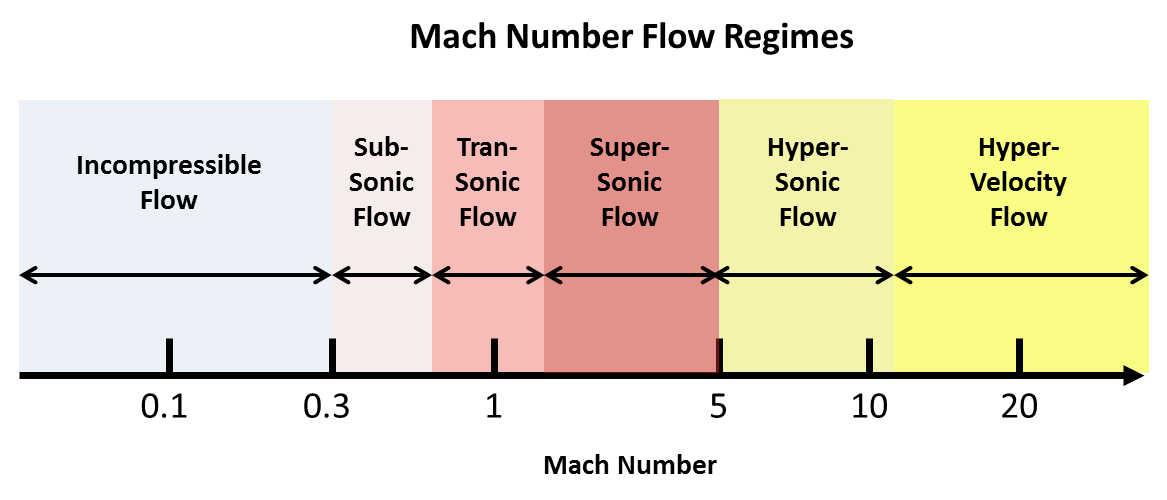
\includegraphics[width=10cm]{Mach-Number-Flow-Regimes}
    \caption{Mach-Number-Flow-Regimes}
\end{figure}

高马赫数流动必须考虑粘性耗散(Viscous dissipation)和压力功(pressure work),模拟高马赫数流动现象必须结合考虑动量和能量传递。在流动过程中热导率$ k $和粘度$ \mu $的变化\textbf{按理想气体}假设来计算。一般使用Sutherland's Law。

\begin{equation}
k = k_{ref}\left( \frac{T}{T_{k,ref}} \right)^{3/2}\frac{T_{k,ref}+S_k}{T+S_k}
\end{equation}

其中,$ k_{ref} $为参考条件下的热导率(\si{\watt\per\meter\per\kelvin}),$ T_{k,ref} $为参考条件下的温度(\si{\kelvin}),$ S_k $为Sutherland常数(\si{\kelvin},每种气体都有自己的常数)。

同理,高马赫流动流体的粘度也可使用Sutherland's Law来计算,\textbf{仅对低压下的单组分气体有效}。

\begin{equation}
\mu = \mu_{ref}\left( \frac{T}{T_{\mu,ref}} \right)^{3/2}\frac{T_{\mu,ref}+S_\mu}{T+S_\mu}
\end{equation}

其中,$ \mu_{ref} $为参考条件下的粘度(\si{\pascal\per\second}),$ T_{\mu,ref} $为参考条件下的温度(\si{\kelvin}),$ S_\mu $为Sutherland常数(\si{\kelvin},每种气体都有自己的常数)。

\section{多孔介质流动}

多孔介质流道所占体积分数为孔隙率$ \varepsilon $,多孔介质单位截面积的体积流率称为Darcy速度(\si{\meter\cubed\per\second\per\square\meter}),孔隙内的平均速度(\si{\meter\per\second})称为The intrinstic average velocity/The average linear velocity,其与Darcy速度可以通过Dupuit–Forchheimer relationship进行关联。为了简便,后续方程中的$ \bm{u} $一般指Darcy速度。(Darcy速度是以整个表征体元为基础计算的,平均速度是以孔隙为基础计算的,所以Darcy速度要小)。

\begin{equation}\label{Dupuit–Forchheimer-relationship}
\bm{u}_{Darcy} = \varepsilon \bm{U}_{ave}
\end{equation}

运用通用的守恒方程导出多孔介质流动的连续性方程:

\begin{equation}
\varepsilon \frac{\partial \rho}{\partial t} + \nabla\cdot(\rho\bm{u}) = 0
\end{equation}

Darcy定律表明,流速和压力梯度成正比,流动的阻力主要是流体的粘性力,Darcy适用于低$ Re $的渗流情况。

\begin{equation}\label{Darcy's-law-2D}
u = -\frac{\kappa}{\mu} \frac{\partial p}{\partial x}
\end{equation}

三维情况下,Darcy定律如下式,其中$ \bm{\kappa} $为渗透率张量。

\begin{equation}\label{Darcy's-law-3D}
\bm{u} = -\frac{\bm{\kappa}}{\mu}\cdot\nabla p
\end{equation}

\subsection{渗透率}

渗透率是由多孔介质几何结构决定的,对于简单和规则的几何结构,我们能够通过几何参数来计算渗透率。对于球形颗粒填充或纤维,渗透率与孔隙率和几何参数有如下关系:

\begin{equation}\label{Carman-Kozeny}
\kappa = \frac{d_p^2\varepsilon^3}{180(1-\varepsilon)^2}
\end{equation}

\subsection{Forchheimer's Equation}
当Darcy流速$ \bm{u} $足够小(通常意味着$ Re<=1 $),流动符合Darcy定律。随着流速逐渐增大,惯性力带来的非线性曳力逐渐增强,在$ 1<=Re<=10 $这个范围内,惯性力的增长都比较平滑。一旦$ Re $足够高,流动的阻力将主要是流体与流道的摩擦力和惯性力。Forchheimer方程扩展了Darcy定律,适用于多孔介质内的快速流动。大量研究表明,从Darcy流动到Darcy–Forchheimer流动的转变发生在$ Re_{\text{local}}>100 $时。

\begin{equation}\label{Forchheimer}
\nabla p = -\frac{\mu}{\kappa}\bm{u} - c_F \kappa^{-1/2}\rho|\bm{u}|\bm{u}
\end{equation}

其中,$ c_F $为无量纲阻力系数,根据Beavers等人的实验总结,阻力系数可按下式计算:

\begin{equation}
c_F = 0.55 \left( 1-5.5\frac{d}{D_e} \right)
\end{equation}

其中,$ d $为颗粒直径,$ D_e $为床层等效直径,$ D_e=2wh/(w+h) $,$ w $为床层宽度,$ h $为床层高度。

除了Forchheimer方程外,Irmay等人也提出了一个关联多孔介质压降的关联式,当$ \beta=150 $,$ \alpha=1.75 $即为著名的Ergun方程:

\begin{equation}\label{Irmay}
\frac{dp}{dx}=-\frac{\beta\mu(1-\varepsilon)^2 u}{d_p^2\varepsilon^3}-\frac{\alpha\rho(1-\varepsilon)u^2}{d_p\varepsilon^3}
\end{equation}

\subsection{Brinkman's Equation}

\begin{equation}\label{Brinkman}
\rho\left[ \frac{1}{\varepsilon}\frac{\partial \bm{u}}{\partial t} + \frac{1}{\varepsilon}\nabla\left( \frac{\bm{u\cdot u}}{\varepsilon} \right) \right] = -\nabla p + \frac{\mu}{\varepsilon}\nabla^2\bm{u}-\frac{\mu}{\kappa}\bm{u}-\frac{c_F\rho}{\kappa^{1/2}}|\bm{u}|\bm{u}
\end{equation}

\subsection{填充床的孔隙率}
大量实验表明,填充床的孔隙率是一个阻尼振荡函数,从壁面处$ \varepsilon=1 $振荡变化到$ 5d_p $处接近稳定。可用经验公式描述孔隙率的变化:

\begin{equation}
\varepsilon=\varepsilon_{\infty}\left[ 1+C e^{\left(-N\frac{y}{d_p}\right)} \right]
\end{equation}

其中,$ y $是距壁面的距离;$ C $,$ N $是经验参数,实验表明$ C=1.4 $,$ \varepsilon_{\infty}=0.4 $时,$ N=5\ \text{or}\ 6 $。

由于壁面附近孔隙率最大,流动过程中流速也最大,这种现象称为“沟流现象”(channeling effect)。








